%% LyX 2.3.4.2 created this file.  For more info, see http://www.lyx.org/.
%% Do not edit unless you really know what you are doing.
\documentclass[english]{article}
\usepackage[utf8]{inputenc}
\usepackage{amsmath}
\usepackage{amssymb}
\usepackage{graphicx}
\def\P{\mathbb{P}}

\makeatletter

%%%%%%%%%%%%%%%%%%%%%%%%%%%%%% LyX specific LaTeX commands.
%% Because html converters don't know tabularnewline
\providecommand{\tabularnewline}{\\}

\makeatother

\usepackage{babel}
\begin{document}
\title{How Opening Schools Influence COVID Infections -- Empirical Evidence
from Czech Republic}
\author{Martin \v Sm\'\i d, Jakub Drbohlav, Milan Zaj\'\i\v{c}ek\thanks{Institute of Information Theory and Automation of the CAS, BISOP}}
\maketitle

\section*{Main findings}
\begin{itemize}
\item Opening of schools in the Czech Republic strongly increases the infection
numbers of students
\item The effect of ordering masks in classrooms is significant in primary
schools and in secondary schools
\item Data do not support the hypothesis that the increase of reported cases
after opening schools is due to more intense testing in schools 
\item Except for kindergartens, data do not support the hypothesis that,
when being out of schools, children are infected elsewhere
\item Simple indicator of safe opening schools can be constructed. 
\item We show that hypothetical opening of schools in the middle of the
pandemics would not overturn the subsequent decreasing trend, yet
it would increase the infections significantly.
\end{itemize}

\section*{Introduction}

Closing schools during the present pandemics is the one of the most
controversial issues. According to epidemiological mainstream, schools
are strong drivers of respiratory diseases {[}cit - Gold, 2021; Stein-Zamir et al., 2020; Torres et al.,2020); see also Forbes et al. (2021); Ismail et al. (2021); Lessler et al. (2021); SAGE (2020);Brauner et al. (2021); Haug et al. (2020), but also Zhu et al. (2020); Zimmerman et al.(2021).{]}; therefore, closing
schools was one of the first governmental reactions to the outburst
of the present pandemic. However, the price we pay for closing schools
is high. Online education is not an equivalent substitute for the
in-person one {[}cit - Di Pietro et al., 2020; Engzell et al., 2020; Maldonado and De Witte,2020{]}; moreover, the isolation of students leaves deficit
in their necessary social contacts {[}cit - Bignardi et al., 2020; ECDC, 2020; Di Pietro et al., 2020;Ravens-Sieberer et al., 2021){]}. Thus, for the society,
decision whether and when to close school means a painful trade-off,
making any decision political rather then scientific; science, however,
has irreplaceable role in giving the best possible (quantitative)
basis for these decisions. 

Unfortunately, it is difficult to evaluate the effect of closing schools
during the present pandemic. The virus was completely unexplored as
it came and its knowledge increased only gradually, so we only gradually
get to know, whether and how differently the virus affects children
in comparison with the rest of the population. To estimate the effect
from running epidemic data is also problematic, mainly because the
counter-epidemic measures are usually being introduced (and released)
together, so it is difficult to distinguish their effects, and even
in cases when the measures are applied in different times, still they
can be assessed only in the context of the other measures applied.
{[}Kulweit 2020{]}, for instance, regards school closure as a very
effective means of curbing the present pandemics; however, it is necessary
to take into account that school closures were usually the first measures
applied, so their measured effect may be overestimated.

In our analysis, we exploit a ``gap'' in this puzzle: the fact that
certain age cohorts of children nearly uniquely correspond to the
degrees of schools and, except for kindergartens, the majority of
children do attend their classes. Thus, it could be expected that
closing (opening) of particular degrees will result in significant
changes in infections in the corresponding cohorts. The other measures,
on the other hand, are usually much less age specific (wearing masks,
bans of gatherings) or are affecting different age cohorts (home office)
so they can be expected not to obscure the effects of school closures.
Later we show that actual data prove us right in both these assumptions
-  the effects of closures are strongly statistically significant
and the data do not exhibit co-linearity.

In the Czech Republic, all kindergartens, primary and secondary schools
had been closed on March 12, 2020, shortly after the first cases of
COVID infection appeared. While the kindergartens had been reopened
without much restriction in the beginning of May, the primary and
the secondary schools were opened during May only in a very limited
regime until the summer vacation. After the vacation, all the schools
had been opened for two weeks nearly without any restriction. Next,
after the overall incidences started to rise, wearing masks in classrooms
had been imposed. In the end of October, after serious increases of
new cases, all the schools had been closed until except
for kindergartens, which remained open until February 27, 2021. Following partial amelioration , first two grades of primary schools had been On November 18, lasty grades of secondary schools on November 25 and, on November 30, whole first degree together with the last grades of primary schools had been fully open, while the rest of primary school grades (6th to 8th) had been open on rotational base. After the Christmas holiday, however, all schools had been closed again except for the first two grades, which remained open until February 27. On April 12th,
2021, kindergartens opened for the final year and the other schools
gradually started to be opened under rotation schemes. See the following
Table for the schedule.

%https://www.idnes.cz/zpravy/domaci/skoly-navrat-deti-studenti-zakladni-skola-andrej-babis-koronavirus-epidemie.A201111_091753_domaci_rapc

%https://www.irozhlas.cz/zpravy-domov/koronavirus-online-v-cesku-cesko-cr-navrat-do-skol-skolstvi-robert-plaga-jan_2011191400_ako

\begin{tabular}{l|c|c|c|c}
Date	&	Kindergartens		&	First degree	&	Second degree	&	Secondary \\
\hline
Mar-13	& volantury	& \multicolumn{3}{c}{closed}\\
May-04	&			&		&	&	\\
May-11	& & &  \multicolumn{2}{c}{last year max. 15 voluntary} \\
May-25    &  & max. 15 voluntary & &  \\
Jun-08	& &  & \\
Jun-26	&	\multicolumn{4}{c}{end of the school year} \\
Sep-01	&	\multicolumn{4}{c}{start of the school year, opened} \\
Sep-17	&	  & \multicolumn{3}{c}{masks ordered in classrooms} \\
Oct-05	&  & & & some closed \\
Oct-14	&  & \multicolumn{3}{c}{closed} \\
Nov-18	&  &  $1^{st}$ $2^{nd}$ open &  &  \\
Nov-25	&  &  & & last year open \\
Nov-30  & & open & rotations, last yr. open & \\
Jan-04	&  & $1^{st}$ $2^{nd}$ open &  closed & closed \\
Feb-27	&    \multicolumn{2}{c}{closed}  & \, & \\
Apr-12  & last years & rotations & &  \\
Apr-26  &  selected open & & &  \\
May-03  &  & & selected rotations &  \\
May-10  & open & & rotations & \\
May-17  & & open with testing & selected open w. t. & \\
May-24 & & & open with testing & open with testing \\
Jun-08 &  & \multicolumn{3}{c}{masks not required in all but 3 regions} \\
Jun-15 &  & \multicolumn{3}{c}{masks not required} \\
June-30 & \multicolumn{4}{c}{end of school year}
\end{tabular}

TBD: viceleta gymnazia: (complication for grammar schools, where equivalents of grades 6-9 in rotations) (these were open from Nov 30)

To evaluate the effects of the closures, we used a simple epidemiological-like
model, in which the infections in the children cohorts depend on the
overall state of epidemic plus the effect of schools, the former summand
being linearly dependent on the product of the current magnitude of
the epidemic and the current overall contact restriction, the latter
being linearly dependent on the the product the current school restrictions
and the number of infected in the cohort in question. We find the
school closures as a whole as a significant inhibitor of the epidemic,
with masks being provably efficient in the primary and secondary schools. 

Next we construct an indicator sub-unit value of which guarantees
keeping the infections in the cohort in question bounded or decreasing,
if the bound is exceeded; this indicator can serve for decisions on
school restriction degree during the epidemic.

Within the Discussion, we also discuss possible alternative explanation
of the infection increases by more extensive testing in schools, and
the hypothesis, that during school closures, children are increasingly
infected elsewhere. We find, that, except for the latter hypothesis
and kindergartens, data do not support these explanations. 

\section*{Methods}

To determine the influence of attending schools of a given kind, we examine the number of reported infections $X_{i,t}$ in the corresponding age cohort for each district $i$ at time $t$. Generally, we assume that these infections depend on the previous-week number of infections, the contact restriction reported two weeks earlier, and the current infectiousness. In addition to the total number of infections in population, we take into account the number of infections in the same district, and the number of infections in the same cohort within the district. See Appendix TBD for the justification of this general model. In addition, we consider the influence of school opening regime on the infection number in the cohort:
\begin{equation}
X_{i,t} = \alpha_i R_t Y_{t-1} + \beta_i R_t Y_{i,t-1} + \gamma R_t X_{i,t-1}
+ S_t X_{i,t-1} + e_{i,t}
\label{eq:x}
\end{equation}
$$
R_t = r_t C_{t-2},\qquad
S_t = r_t (\nu N_{t-1} + \mu M_{t-1} + \varrho T_{t-1} + \nu^\star N^\star_{t-1}
+ \mu^\star M^{\star}_{t-1} + \varrho^\star T^\star_{t-1} 
)
$$
for each $i$ and $t$. Here, $Y_t$ is the number of overall infections within the population at $t$, $Y_{i,t}$ is the number of infections within the $i$-th district at $t$, $N_t$, $M_t$, $T_t$ evaluate the degree of school opening without masks, with masks, with weekly rotations (with masks on), respectively (zero means all classes closed, one means all classes opened), $N^\star_t$, $M^\star_t$, $T^\star_t$ stand for for degree of opening without--, with masks, with rotations , respectively, with the addition that students are regularly tested at schools,  and $e_{i,t}$ is the error term. Finally $r_t$ is the (predicted) degree of infectiousness and $C_t$ is the contact restriction at $t$, see  Appendix TBD for details.

We estimate the impact of schools four ways: by comparing two sub-cohorts of the examined cohort assuming them to follow (\ref{eq:x}) either with the same or with different school regime coefficients $\nu,\mu,\dots,\varrho^\star$, by estimating parameters from (\ref{eq:x}) applied to the whole cohort and, finally, by estimating the parameters from  (\ref{eq:x}) with homogeneous impact of districts.

{\em Comparison of two sub-cohorts with different regime parameters.} Here we consider two sub-cohorts of comparable size, the $j$-th one following its own version of (\ref{eq:x}):
$$
X^j_{i,t} = \alpha^j_i R_t Y_{t-1} + \beta^j_i R_t Y_{i,t-1} + \gamma^j c_j R_t X_{i,t-1}
+ S^j_t c_j X_{i,t-1} + e^j_{i,t}
$$
$$
S^j_t = r_t [\nu^j N^j_{t-1} + \mu^j M^j_{t-1} + \varrho^j R^j_{t-1} + \mu^{\star j} M^{\star  j}_{t-1} + \nu^{\star j} N^{\star j}_{t-1} +  \varrho^{\star j} R^{\star j}_{t-1} ],
$$
where $c_j$ is the relative size of the $j$-th sub-cohort with respect to whole cohort. By subtracting, we get 
\begin{equation}
\frac{X^{1}_{i,t}}{c_{1}} - \frac{X^{2}_{i,t}}{c_{2}} = \alpha'_i R_t Y_{t-1} + \beta'_i R_t Y_{i,t-1} 
+ \gamma' R_t X_{i,t-1} + D_t X_{i,t-1} + e'_{i,j,t}, \qquad D_t = S^1_t - S^2_t
\label{eq:dif}
\end{equation}
Clearly, for (\ref{eq:dif}) to be estimable, at least one pair of variables $(N^1,N^2),\dots,(T^{\star 1},T^{\star 2})$ has to differ sufficiently. For instance, this was the case for kindergartens, where the only regimes having occurred were opening without masks ($N^1_t = N^2_t = 1$), opening only for the last years ($N^1_t=1,N^2_t=0$) and closure ($N^1_t = N^2_t = 0$), so both $\nu^1$ and $\nu^2$ are estimable from
$
D_t=r_t (\nu^1 N^1_{t-1} - \nu^2 N^2_{t-1})  
$.
Note that the results of this estimation can also be used to test the null hypothesis that the corresponding regime has no influence on infections, which will be rejected by significant values of either $\nu^{1}$ or $\nu^2$.\footnote{The significance level has to be corrected here.}

{\em Comparison of two sub-cohorts with the same regime parameters.} If we decrease the generality of the model (\ref{eq:dif}) by assuming that $\nu^1 = \nu^2 = \nu$, $\dots$, $\varrho^{\star 1} = \varrho^{\star 2} = \varrho^{\star}$, we get
$$
D_t = r_t [\nu (N^1_{t-1}-N^2_{t-1}) + \dots + \varrho^\star (R^{\star 1}_{t-1}-R^{\star 2}_{t-1})  ] 
$$
from which we can estimate $\nu, \dots, \varrho^\star$ with the advantage that the variables and coefficients for which the regime is the same, cancel out, so our estimate is independent both of these parameters and on the choice of corresponding regime covariates, which we have are set subjectively sometimes, for instance when the schools are opened with another additional restrictions. Clearly, only the coefficients for which the corresponding covariates differ at least for some time can be estimated this way. Again, the estimation may serve for proof that the opening in the particular regime influences infections.

{\em Estimation of (\ref{eq:x}) for the whole cohort.} For the coefficients corresponding to regimes, which had never differed between the sub-cohorts, there is nothing to do but to estimate them directly from (\ref{eq:x}). 

Finally, to get global results rather than the district-level ones, we  decrease the generality of (\ref{eq:x}) and assume a {\em homogeneous model}:
\begin{equation}
X_{i,t} = \alpha h d_i R_t Y_{t-1} + \beta h R_t Y_{i,t-1} + \gamma R_t X_{i,t-1}
+ S_t X_{i,t-1} + \epsilon_{i,t},
\label{eq:linear}
\end{equation}
Here, $h$ is the relative size of the examined cohort with respect to the rest of the population and $d_i$ is the relative size of the $i$-th district's population.
By summing (\ref{eq:linear}) over $i$, we get 
\begin{equation}
X_{t} =  \omega h R_t Y_{t-i}
+ (\gamma R_t +  S_{t})X_{t-1} + \epsilon_{t}, \qquad \omega = \alpha +\beta,
\label{eq:xss}
\end{equation}
where $X_t$ is number the overall cohort infections. The equation (\ref{eq:xss}) may be alternatively interpreted as
\begin{multline*}
\P[\text{infection in cohort at $t$}]
\\
\doteq \omega R_t  \P[\text{overall infection at $t-1$}] + (\gamma R_t +  S_{t}) \P[\text{infection in cohort at $t-1$}]
\end{multline*}
(to see it, divide (\ref{eq:xss}) by the cohort size).\footnote{Similarly, we can interpret 
(\ref{eq:linear}) as
\begin{multline*}
\P[\text{infection in cohort in district $i$ at $t$}]
\\
\doteq \alpha R_t \P[\text{overall infection at $t-1$}]
+\beta R_t \P[\text{infection in district $i$ at $t-1$}] \\
+(\gamma R_t + S_{t}) \P[\text{infection in cohort in $i$ at $t-1$}]
\end{multline*}
where $h_i$ is the relative size of the cohort within district $i$ and $s_i$ is the relative size of the $i$-th district population, both with respect to the whole population (to see it, it suffices to divide (\ref{eq:linear}) by the cohort size).} 
\def\defined{\stackrel{\text{def}}{=}}

Finally, if we divide (\ref{eq:xss}) by $X_{t-1}$, we get the relative growth of infections within the cohort:
$$
\rho_t \defined \frac{X_{t}}{X_{t-1}}=G_t + S_t+ \eta_t
\qquad G_t = R_t \left[\omega \frac{h Y_{t-1}}{X_{t-1}}+\gamma \right],\qquad
\eta_t=\frac{\epsilon_t}{X_{t-1}}
$$
from which we can distinguish the part of the growth caused by school opening (quantified by $S_t$) from that originated outside schools ($G_t$).



\section*{Data}

In the Czech Republic, each September first, children who completed
their sixth year are obliged to enter the first grade of an elementary
school. When the parents wish, a child who is six as late as by the
end of the year can enter the first class, too, some children, on
the other hand, start their school later for various, mostly developmental,
reasons. If we neglect these exceptions, we can conclude that the
first year pupils are six or seven; consequently the first degree
(first five grades) pupils belong to the age cohort $6-11$. The second
degree (the sixth to the ninth year) students to the cohort $11-15$.
Finally, the students of secondary schools, which typically take four
year in the Czech Republic, belong to the cohort $15-19$. The lowest
age for admission to a kindergarten is three, so the the vast majority
of children attending kindergartens falls into the cohort $3-6$.
For simplicity we assume that the frontier one-year cohorts split
by half between the competing school categories, so the infections
happening in the cohort split by two between each category. 

Thus the number of cases by pre-school children over week $t$ in
the $i$-th district will be $X_{i,t}^{1}=Z_{i,t}^{3}+Z_{i,t}^{4}+Z_{i,t}^{5}+\frac{1}{2}Z_{i,t}^{6}$,
the number by the first degree $X_{i,t}^{2}=\frac{1}{2}Z_{i,t}^{6}+Z_{i,t}^{7}+\dots+\frac{1}{2}Z_{i,t}^{11}$,
by the second degree $X_{i,t}^{3}=\frac{1}{2}Z_{i,t}^{11}+Z_{i,t}^{12}+\dots+\frac{1}{2}Z_{i,t}^{15}$
and that by the secondary schools $X_{i,t}^{4}=\frac{1}{2}Z_{i,t}^{15}+Z_{i,t}^{16}+\dots+\frac{1}{2}Z_{i,t}^{19},$where
$Z_{i,t}^{j}$ is the number of cases by the $j$-year old individuals
in the $i$-th district. The values $Z^j_{i,t}$ from the public dataset by the Czech Ministry of
Health, namely the anonymized person-level list of reported infections
(cit osoby.htm) including, among other things, the date of reporting
the infection and the age. The series $Y_t$ and $Y_{i,t}$ are computed by aggregation.

The values of contact reduction $C_t$ were taken from the longitudinal sociological survey \cite{paqcovid}. The trend $r_{t}$ is computed by double exponential smoothing of series
$\frac{Y_{t}/Y_{t-1}}{C_{t-1}}$ with parameter $\alpha=0.2,\gamma=0.5$.  

The values of $N$ and $M$ are estimated from publicly available
sources, mostly from resolutions of the Czech government concerning
school attendance, which have been put into effect through decrees
of the Ministry of Education (see the electronic supplement for
details). Yet first cases appeared in teh beginning of March, 2020, 
only weeks starting from April 6th, 2020 are taken into
account, as we regard the previous epidemic data as noisy, unreliable
and suffering from small sample properties. The last values correspond
to the week staring on April 5th, 2021. The values of $N$ were set
to $1$ if the school was open without any restrictions, and to $0$ if they were closed or masks were ordered. Similarly, the values of $M$ were put to $1$ if the school was fully open with masks in classroom and to $0$ if they were closed or open with masks. If the school type was open only partially, we either set $N$ (or $M$) to a fractional value if a reasonable way to determine the value existed, otherwise the observation was excluded. We also 
excluded observations corresponding to holidays and the weeks with no
more than two possible school days. The list of values $N$ and $M$ finds itself in the Table
in Appendix together with the notes on how we determined fractional
values and reasons of observation exclusions. The following table
summarizes our data-set. 

We identified three opportunities for sub-cohort comparison. The first was opening only the first two grades of primary schools from January 4th until February 24th, 2021 while the first of the primary schools were closed. Here we compared cohorts $X_{i,t}^{2,1}=\frac{1}{2}Z_{i,t}^{6}+Z_{i,t}^{7}+\frac{1}{2}Z_{i,t}^{8}$, corresponding to the first two grades, with  $X_{i,t}^{2,2}=\frac{1}{2}Z_{i,t}^{9}+Z_{i,t}^{10}+\frac{1}{2}Z_{i,t}^{11}$. As the masks were ordered, we put $M^{1}=1$, $M^{2}=0$, $N^1=N^2=0$ during the mentioned weeks, while, for the rest of the observations, $M^{1}=M^{2}$, $N^1=N^2$ as the conditions were identical for both the cohorts. As there was no difference of the $N$'s, we could estimate only $\delta$ but not $\gamma$. 

In the second case we compared the cohort corresponding to the last years of the primary schools (half of 14 year plus the half of the 15 year) with the closest corresponding not overlapping cohort (half of 12's plus the half of 13's). The last years were opened on May 11th, 2020, on voluntary basis for groups of at most 15 students, while the rest of the second degree remained closed until May 25, so there were two weeks for comparison.  Further, on November 30. 2020. the last years were opened while the rest went to school on the rotational basis; this state took place until Christmas (three weeks). Here we put $M^1=0.4$, $M^2=0$ for the spring three weeks (masks were not ordered) and $N^1=1$, $N^2=0.5$ for the autumn three weeks (otherwise the conditions were identical), so we could estimated both $\gamma$ and $\delta$.

Finally, we compared the cohort corresponding to the last years of secondary schools with the closest cohort from secondary schools for the three weeks starting from November 30, when the last years were open while the rest of secondary schools were closed. As masks were ordered, we put $M^1=1$, $M^2=0$ during this weeks with the $N$'s and the rest of $M$'s identical, being able to estimate only $\delta$.




\section*{Results }

The following Table shows results of estimation of (\ref{eq:dif}) (differences of sub-cohorts) with different and identical regime parameters, of (\ref{eq:x}) (single model for the subcohort) and of (\ref{eq:linear}) (homogenous model).

\begin{tabular}{cc|cccc} \multicolumn{2}{c}{Model}& Kindergartens & First degree & Second degree & Secondary \\ \hline Sub-cohort & 1 & last year & 1st and 2nd yr. & 9th year & 4th year \\  & 2 & 5 year old & 4th and 5th yr. & 7th year  & 2nd year \\ \hline 
Comparison &$\nu^1$& $0^{}(0.03)$&&&\\
different &$\nu^2$& $-0.01^{}(0.03)$&&&\\
($w=30\%$) &$\mu^1$&& $0.15^{***}(0.01)$& $0.19^{***}(0.04)$& $0.16^{***}(0.06)$\\
&$\mu^2$&& $0.29^{***}(0.04)$&& $0.32^{***}(0.08)$\\ 
&$\rho^2$&&& $0.13^{**}(0.06)$&\\ \hline
Comparison &$\mu$&& $0.18^{***}(0.02)$&& $0.19^{***}(0.06)$\\
same ($w=55\%$) &$\mu-\rho$&&& $0.04^{}(0.05)$&\\ \hline
Whole &$\nu$& $0^{}(0)$& $0.33^{***}(0.04)$& $0.68^{***}(0.04)$& $0.91^{***}(0.04)$\\
cohort &$\mu$&& $0.26^{***}(0.02)$& $0.16^{***}(0.03)$& $0.29^{***}(0.04)$\\
($w=10\%$) &$\rho^\star$&&&&\\
&$\mu^\star$&& $0.12^{***}(0.02)$& $0.12^{***}(0.02)$& $0.22^{***}(0.03)$\\
&$\nu^\star$&& $0.05^{}(0.03)$& $0.17^{***}(0.03)$& $0.31^{***}(0.04)$\\
&$\gamma$& $0.08^{***}(0.01)$& $-0.17^{***}(0.03)$& $-0.14^{***}(0.03)$& $-0.22^{***}(0.04)$\\ \hline
Homogenous &$\nu$& $-0.01^{***}(0)$& $0.32^{***}(0.04)$& $0.65^{***}(0.04)$& $0.95^{***}(0.04)$\\ 
($w=5\%$) &$\mu$&& $0.25^{***}(0.02)$& $0.15^{***}(0.03)$& $0.32^{***}(0.04)$\\ 
&$\rho^\star$&& $0.07^{***}(0.01)$& $0.01^{}(0.03)$&\\ 
&$\mu^\star$&& $0.07^{***}(0.02)$& $0.12^{***}(0.02)$& $0.19^{***}(0.03)$\\ 
&$\nu^\star$&& $-0.02^{}(0.03)$& $0.13^{***}(0.03)$& $0.34^{***}(0.04)$\\ 
&$\alpha$& $0.02^{**}(0.01)$& $0.07^{***}(0.02)$& $0.1^{***}(0.03)$& $0.19^{***}(0.03)$\\
&$\beta$& $0.14^{***}(0.01)$& $0.48^{***}(0.02)$& $0.63^{***}(0.03)$& $0.44^{***}(0.03)$\\
&$\gamma$& $0.15^{***}(0.01)$& $-0.05^{**}(0.03)$& $-0.07^{**}(0.03)$& $-0.16^{***}(0.03)$\\ 
\end{tabular}
\begin{tabular}{l|ccc} Parameter & First degree & Second degree & Secondary \\ \hline 
$\nu$& $0.33(0.04)$& $0.67(0.04)$& $0.93(0.04)$\\
$\mu$& $0.21(0.02)$& $0.17(0.04)$& $0.22(0.06)$\\
$\rho$&& $0.13(0.06)$&\\
$\rho^\star$& $0.09(0.02)$& $0.03(0.03)$&\\
$\mu^\star$& $0.11(0.02)$& $0.12(0.02)$& $0.21(0.03)$\\
$\nu^\star$& $0.03(0.03)$& $0.15(0.03)$& $0.32(0.04)$\\
$\gamma$& $-0.05(0.03)$& $-0.07(0.03)$& $-0.16(0.03)$\\
$\omega$& $0.55(0.04)$& $0.73(0.06)$& $0.63(0.06)$\\
\end{tabular}

Further, we aggregated the parameters by an average weighted by values shown in the first column and with upper estimates of standard errors.
\begin{tabular}{l|ccc} Parameter & First degree & Second degree & Secondary \\ \hline 
$\nu$& $0.33(0.04)$& $0.67(0.04)$& $0.93(0.04)$\\
$\mu$& $0.21(0.02)$& $0.17(0.04)$& $0.22(0.06)$\\
$\rho^\star$& $0.09(0.02)$& $0.08(0.04)$&\\
$\mu^\star$& $0.11(0.02)$& $0.12(0.02)$& $0.21(0.03)$\\
$\nu^\star$& $0.03(0.03)$& $0.15(0.03)$& $0.32(0.04)$\\
$\gamma$& $-0.05(0.03)$& $-0.07(0.03)$& $-0.16(0.03)$\\
$\omega$& $0.55(0.04)$& $0.73(0.06)$& $0.63(0.06)$\\
\end{tabular}





The results strongly indicate the influence of opening corresponding
school categories and they also indicate that wearing masks reduces
infections significantly.
These results are further illustrated by the following charts.

\includegraphics[width=5cm]{nomasks.eps} \includegraphics[width=5cm]{withmasks.eps}

\includegraphics[width=5cm]{general.eps}

In a hypothetical situation when the probability of contagion is the same all in the districts and cohorts, the heights columns and their sections are comparable across charts, up to a constant, the probability of contagion in the corresponding cohorts, the sections of the columns displaying the contributions of the individual sources (overall situation, own district and school, when open).


To give the reader an idea about quantities in question, we further
plotted predictions of the ``as usual'' model for all the cohorts,
see the following Figure

\begin{tabular}{|c|c|}
\hline 
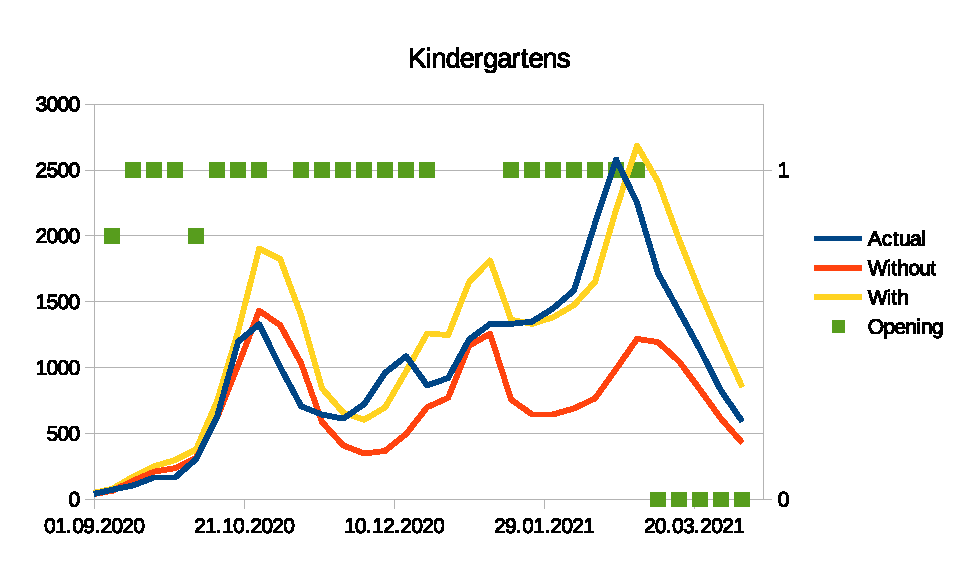
\includegraphics[scale=0.3]{k} & \includegraphics[scale=0.3]{fg}\tabularnewline
\hline 
\hline 
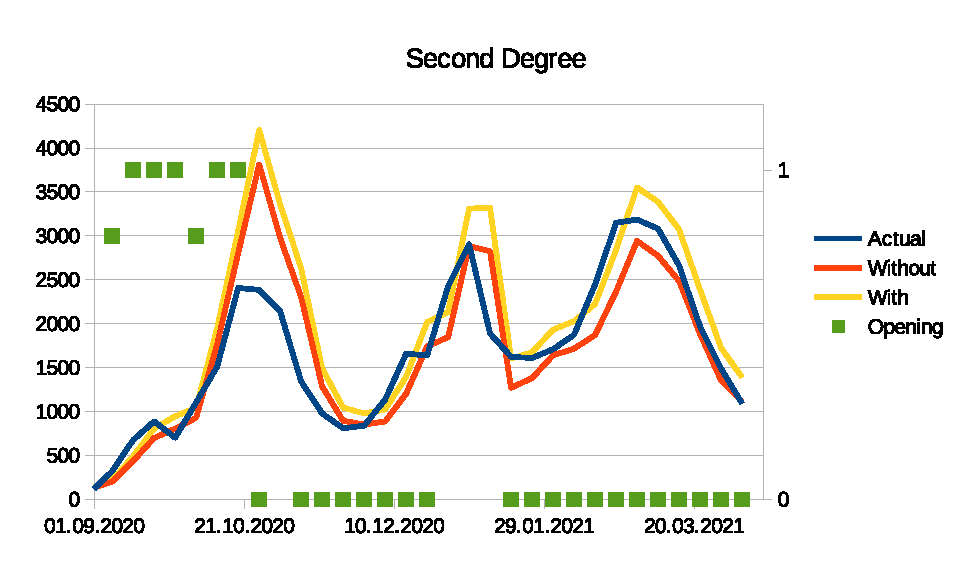
\includegraphics[scale=0.3]{sg} & \includegraphics[scale=0.3]{sec}\tabularnewline
\hline 
\end{tabular}

The graphs show one-week predictions of $Y_{t}^{i}$ with-- and without
schools (fully) open, i.e. with $S_{t-1}=1$, $S_{t-1}=0$, respectively,
and with $M$ set according to the usual manner. In addition, actual
(observed) numbers and the degree of opening schools one week before
(values of $S_{t-1}^{i}$) are depicted. It can be seen that, according
to the model, full opening of schools (in a usual manner) at least
doubles the new cases in corresponding except for the second degrees;
however, it is important to keep in mind the insignificance of results
for the primary schools. 

Finally, we evaluated index $\rho_{t}$ for all the types during the
school year 2020/21. Recall that $\rho_{t}$ is an indicator of safe
opening of schools, whose value below $1$ indicate that the cases
in the corresponding cohort will not rise. Recall also that the indicator
is a sum of a part dependent on the outside epidemic (indexed by $\alpha$)
and the part dependent on the degree of opening of schools (indexed
by $\gamma)$. The following graphs show the values of the index through
time (with the the true degree of opening)

\begin{tabular}{|c|c|}
\hline 
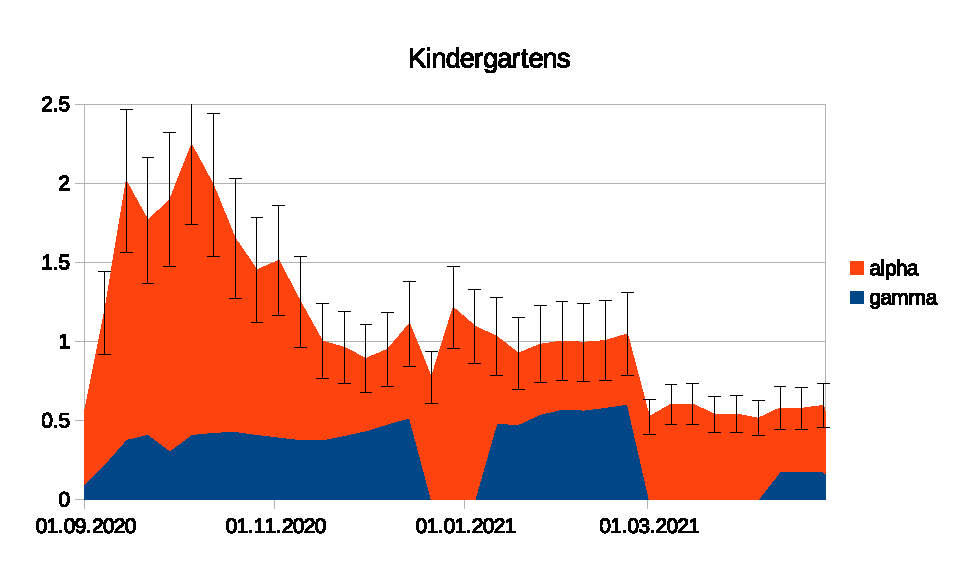
\includegraphics[scale=0.3]{rhokreal} & 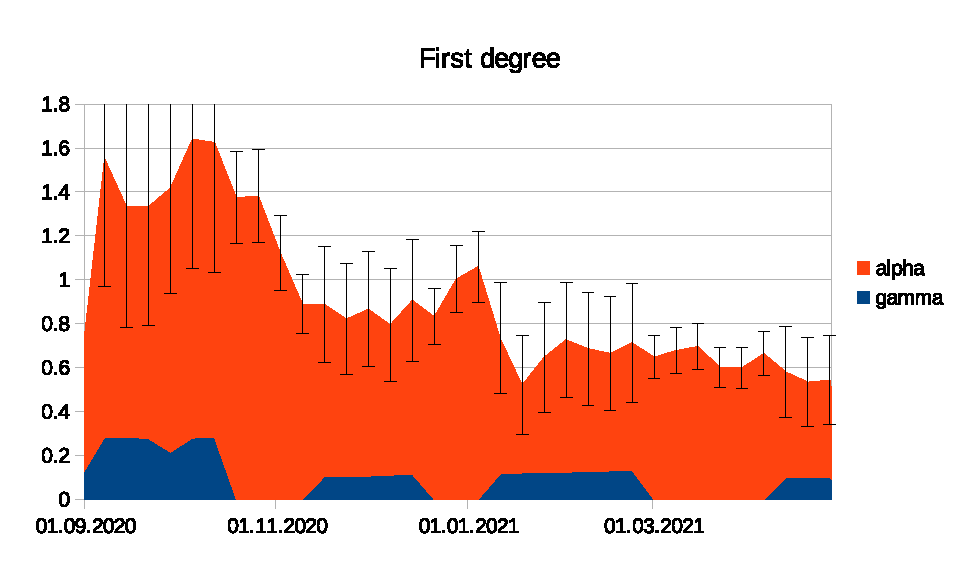
\includegraphics[scale=0.3]{rhofdreal}\tabularnewline
\hline 
\hline 
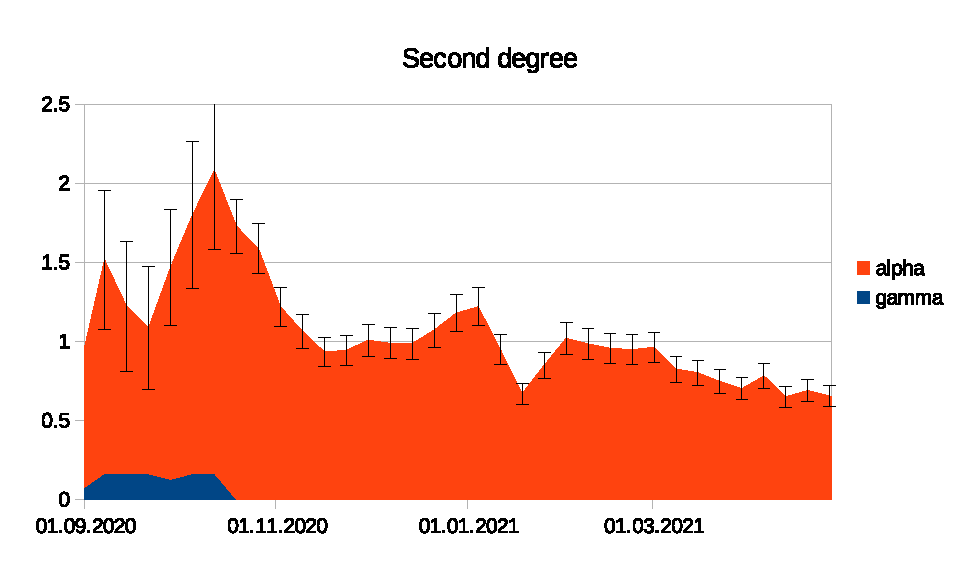
\includegraphics[scale=0.3]{rhosdreal} & \includegraphics[scale=0.3]{rhosecreal}\tabularnewline
\hline 
\end{tabular}

Here we see that, while the closure of all types of schools may have
helped in Autumn, their closure, or not opening at least in some restricted
mode, in March seems strict. However, it should be stressed that the
indicators $\rho_{t}$ speaks only about the growth at a given time;
if the schools were open, however, the numbers of infected students
would rise, possibly amplifying the effect. To examine this, we modeled
the hypothetical situation in which all the schools were all open
(in a usual manner, i.e. with masks wherever except for kindergartens),
on March 1, which was the time when all the schools had been closed
in reality. In our forecast, we assumed the numbers of cases outside
the examined cohorts to be as in reality while the numbers in the
cohorts were computed according to the ``as usual'' model (i.e.
we neglect a possible increase outside schools due to additional infections
there). The results can be seen in the following charts.

\begin{tabular}{|c|c|}
\hline 
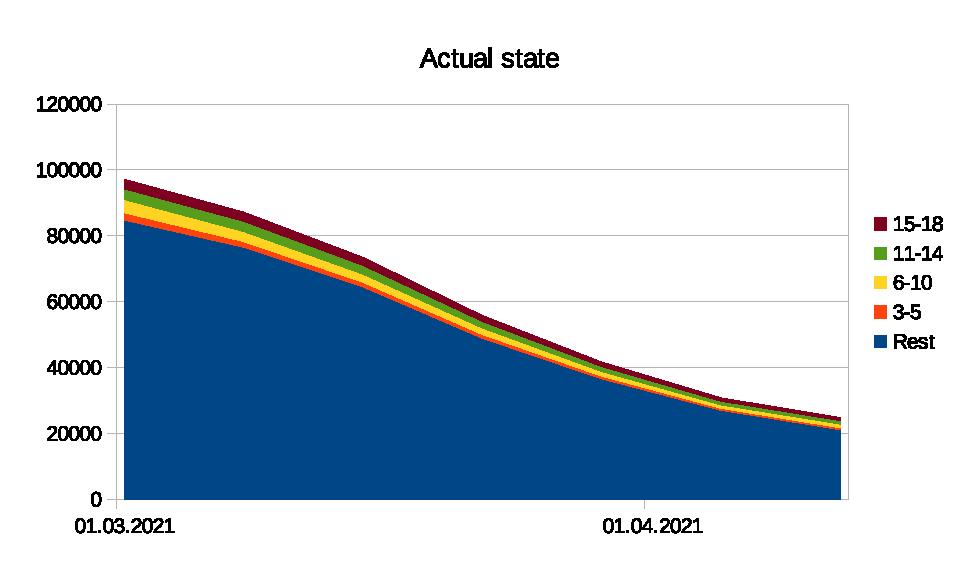
\includegraphics[scale=0.3]{marchclosed} & 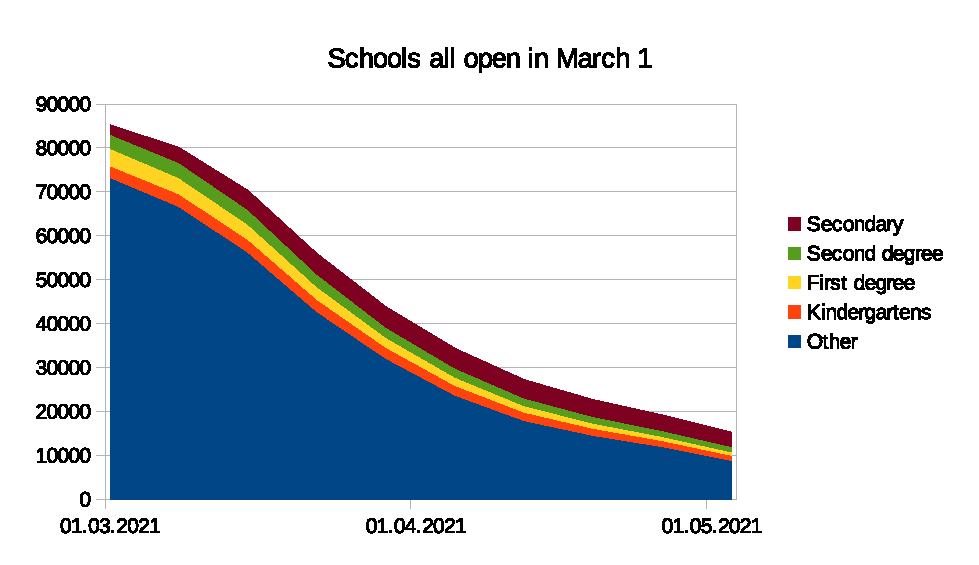
\includegraphics[scale=0.3]{marchopened}\tabularnewline
\hline 
\end{tabular}

We see in the chart, that the contribution of such opening is quite
significant and, yet it does not seem to overturn the decreasing trend
of the epidemic, it probably would, if other areas acted according
the same logic and opened too. The result however shows that, if opening
schools were politically prioritized, it would not make much harm.

\section*{Discussion}

In our honest opinion, our results convincingly prove the strong influence
of in-class education over various types of schools on the epidemic
spread, as well as its reduction by wearing masks in rooms. However,
our study has limitations. First of all it is the shortage of data.
Most of the weeks we examine the schools have been closed, and when
they were opened, mostly with masks, which clearly complicates quantification
of their influences. Therefore, the quantitative results should be
taken with slight caution.

Further, there is a determinant of children infections not taken into
account in our analysis: encounters with teachers, which can be significant
(TBD cite Neruda et al). This influence could be taken into account
by adding another coefficient into (\ref{eq:awls}); however, due
to the data shortage, there would be little chance for significant
results.

Further we discuss two arguments, often in discussions on schools:
that children, not going to schools, are infected anyway in other
environments, and that this influence of schools is spurious due to
more extensive testing of students attending schools in person, (yet,
in the examined period, no preventive testing in schools took place).
In our model, the former hypothesis would mean that, in addition to
fraction $\alpha^{i}Q_{t}$infected outside schools, $k^{i}(1-S_{t-1}^{i})Q_{t}$
for some $k^{i}$ would be infected. The latter hypothesis, on the
other hand, could be expressed as $Y_{t}^{i}=(c+S_{t-1}^{i}d^{i})X_{t}^{i}$
for some $d^{i}$. Both the hypotheses can thus be examined by estimating
a variant of the ``as usual'' model
\[
P_{t}^{i}\doteq\beta^{i}Q_{t}+\gamma^{i}U_{t}+\phi^{i}W_{t}^{i}+\eta_{t},\qquad W_{t}^{i}=Q_{t}S_{t-1}^{i};
\]
with values of $\phi^{i}<0$ speaking for the first hypothesis (children
are infected anyway), the values $\phi>0$ for the second one (there
is higher chance to be tested at school). The results of this estimation
can be found in the following Table 

\begin{tabular}{c|cccc|c}
& Kindergartens  & First degree & Second degree & Secondary & Primary \\ 
& no masks & masks & masks & masks & masks\\
\hline
$\beta$	& $0.535^{***}(0.075)$	& $0.557^{***}(0.0385)$	& $0.846^{***}(0.0454)$	& $0.578^{***}(0.0484)$	& $0.49^{***}(0.0466)$		\\ $\gamma$	& $0.49^{***}(0.058)$	& $-0.74^{}(0.467)$	& $-0.17^{}(0.339)$	& $0.4^{*}(0.22)$	& $0.35^{***}(0.047)$		\\ $\phi$	& $-0.29^{***}(0.098)$	& $0.64^{**}(0.322)$	& $0.3^{}(0.357)$	& $0.04^{}(0.305)$	& $0.04^{}(0.093)$		\\ \hline 
\end{tabular}

We can see from the table, that, for the two oldest cohorts, $\phi$
is insignificant, while, for the kindergarten cohort, results support
the hypothesis ``infected instead''. For the first degree cohort,
data suggest the ``over-tested'' hypothesis; here, however, the
result is unintuitive ($\gamma<0)$, which is probably due co-linearity
(VIR is nearing 20), invalidating the estimate of $\phi$, too. Thus,
only ``infected instead'' alternative in kindergartens should be
taken into account. However, the results are comparable here: the
following charts show the ``safety criterion'' $\rho_{t}$, which
is now changed to 

\[
\rho_{t}:=\rho_{t}^{\alpha\psi}+\rho_{t}^{\gamma}<\rho_{0},\qquad\rho_{t}^{\alpha\psi}=r_{t}(\alpha^{i}C_{t-1}+\psi^{i}S_{t-1}^{i})\frac{Y_{t-1}}{\max(Y_{t-1}^{i},y_{0})},\qquad\psi^{\acute{\imath}}=\frac{s^{i}}{s}\phi^{i}
\]
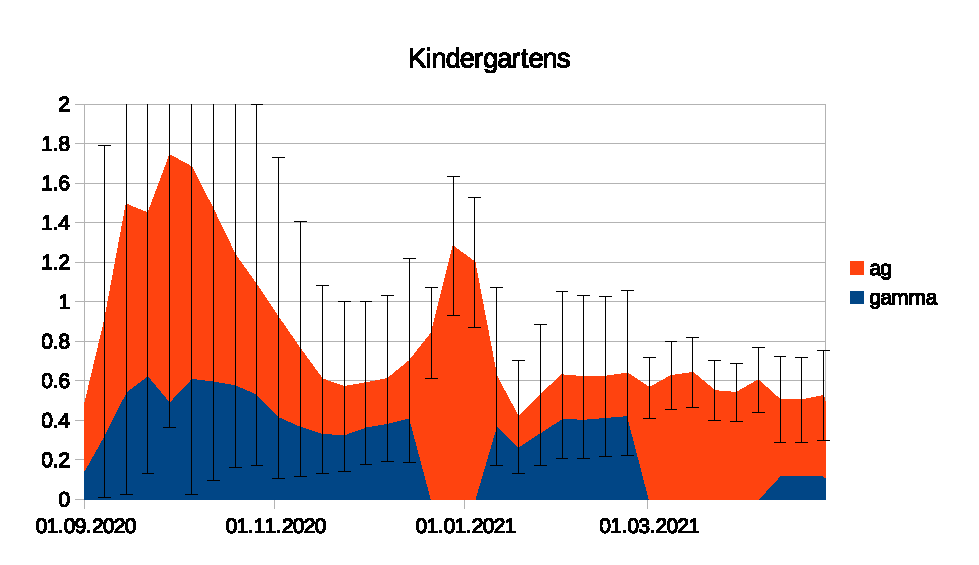
\includegraphics[scale=0.3]{rhokpsi}

\section*{Questions/Ideas}
\begin{itemize}
\item Not split primary schools (and present degrees only as secondary results)?
\end{itemize}

\section*{Appendix}

\begin{center}
\begin{table}
\small
\begin{tabular}{c|cccccccc}																																						
Date	&	\multicolumn{2}{c}{Kindergartens}		&	\multicolumn{2}{c}{First degree}	&	\multicolumn{2}{c}{Second degree}	&	\multicolumn{2}{c}{Secondary}			\\ \hline																										
	&	$N^1$		&	$M^1$											&	$N^2$		&	$M^2$			&	$N^3$		&	$M^3$			&	$N^4$		&	$M^4$				\\ \hline
06-Apr-20	&	$0$		&	$0$											&	$0$		&	$0$			&	$0$		&	$0$			&	$0$		&	$0$				\\
13-Apr-20	&	$0$		&	$0$											&	$0$		&	$0$			&	$0$		&	$0$			&	$0$		&	$0$				\\
20-Apr-20	&	$0$		&	$0$											&	$0$		&	$0$			&	$0$		&	$0$			&	$0$		&	$0$				\\
27-Apr-20	&	$0$		&	$0$											&	$0$		&	$0$			&	$0$		&	$0$			&	$0$		&	$0$				\\
04-May-20	&	$1$		&	$0$											&	$0$		&	$0$			&	$0$		&	$0$			&	$0$		&	$0$				\\
11-May-20	&	$1$		&	$0$											&	$0$		&	$0$			&	$0^{ad}$		&	$0.1$			&	$0^{d}$		&	$0.25$				\\
18-May-20	&	$1$		&	$0$											&	$0$		&	$0$			&	$0^{ad}$		&	$0.1$			&	$0^{d}$		&	$0.25$				\\
25-May-20	&	$1$		&	$0$											&	$0^{a}$		&	$0.4$			&	$0^{ad}$		&	$0.1$			&	$0^{ad}$		&	$0.1$				\\
01-Jun-20	&	$1$		&	$0$											&	$0^{a}$		&	$0.4$			&	$0^{ad}$		&	$0.1$			&	$0^{ad}$		&	$0.1$				\\
08-Jun-20	&	$1$		&	$0$											&	$0^{a}$		&	$0.4$			&	$0^{a}$		&	$0.4$			&	$0$		&	$0$				\\
15-Jun-20	&	$1$		&	$0$											&	$0^{a}$		&	$0.4$			&	$0^{a}$		&	$0.4$			&	$0$		&	$0$				\\
22-Jun-20	&	$1$		&	$0$											&	$0^{a}$		&	$0.4$			&	$0^{a}$		&	$0.4$			&	$0$		&	$0$				\\
29-Jun-20	&	$\times^{e}$		&												&	$\times^{e}$		&				&	$\times^{e}$		&				&	$\times^{e}$		&					\\
	&	$\vdots$		&												&	$\vdots$		&				&	$\vdots$		&				&	$\vdots$		&					\\
																																						
																																						
																																						
																																						
																																						
																																						
24-Aug-20	&	$\times^{e}$		&												&	$\times^{e}$		&				&	$\times^{e}$		&				&	$\times^{e}$		&					\\
31-Aug-20	&	$0.8^{a}$		&	$0$											&	$0.8^{b}$		&	$0$			&	$0.8^{b}$		&	$0$			&	$0.8^{b}$		&	$0$				\\
07-Sep-20	&	$1$		&	$0$											&	$1$		&	$0$			&	$1$		&	$0$			&	$1$		&	$0$				\\
14-Sep-20	&	$1$		&	$0$											&	$0.6^{I}$		&	$0.4$			&	$0.6^{I}$		&	$0.4$			&	$0.6^{I}$		&	$0.4$				\\
21-Sep-20	&	$1$		&	$0$											&	$0$		&	$1$			&	$0$		&	$1$			&	$0$		&	$1$				\\
28-Sep-20	&	$0.8^{a}$		&	$0$											&	$0^{b}$		&	$0.8$			&	$0^{b}$		&	$0.8$			&	$0^{b}$		&	$0.8$				\\
05-Oct-20	&	$1$		&	$0$											&	$0$		&	$1$			&	$0$		&	$1$			&	$\times^{j}$		&					\\
12-Oct-20	&	$1$		&	$0$											&	$\times^{h}$		&				&	$\times^{h}$		&				&	$\times^{h}$		&					\\
19-Oct-20	&	$1$		&	$0$											&	$0$		&	$0$			&	$0$		&	$0$			&	$0$		&	$0$				\\
26-Oct-20	&	$1$		&	$0$											&	$\times^{g}$		&				&	$\times^{g}$		&				&	$\times^{g}$		&					\\
02-Nov-20	&	$1$		&	$0$											&	$0$		&	$0$			&	$0$		&	$0$			&	$0$		&	$0$				\\
09-Nov-20	&	$1$		&	$0$											&	$0$		&	$0$			&	$0$		&	$0$			&	$0$		&	$0$				\\
16-Nov-20	&	$1$		&	$0$											&	$\times^{k}$		&				&	$0$		&	$0$			&	$0$		&	$0$				\\
23-Nov-20	&	$1$		&	$0$											&	$\times^{k}$		&				&	$0$		&	$0$			&	$\times^{k}$		&					\\
30-Nov-20	&	$1$		&	$0$											&	$0$		&	$1$			&	$0^{l}$		&	$0.625$			&	$0^{d}$		&	$0.25$				\\
07-Dec-20	&	$1$		&	$0$											&	$0$		&	$1$			&	$0^{l}$		&	$0.625$			&	$0^{d}$		&	$0.25$				\\
14-Dec-20	&	$1$		&	$0$											&	$0$		&	$1$			&	$0^{l}$		&	$0.625$			&	$0^{d}$		&	$0.25$				\\
21-Dec-20	&	$\times^{f}$		&												&	$\times^{f}$		&				&	$\times^{f}$		&				&	$\times^{f}$		&					\\
28-Dec-20	&	$\times^{f}$		&												&	$\times^{f}$		&				&	$\times^{f}$		&				&	$\times^{f}$		&					\\
04-Jan-21	&	$\times^{f}$		&												&	$\times^{f}$		&				&	$\times^{f}$		&				&	$\times^{f}$		&					\\
11-Jan-21	&	$1$		&	$0$											&	$0^{c}$		&	$0.4$			&	$0$		&	$0$			&	$0$		&	$0$				\\
18-Jan-21	&	$1$		&	$0$											&	$0^{c}$		&	$0.4$			&	$0$		&	$0$			&	$0$		&	$0$				\\
25-Jan-21	&	$1$		&	$0$											&	$0^{c}$		&	$0.4$			&	$0$		&	$0$			&	$0$		&	$0$				\\
01-Feb-21	&	$1$		&	$0$											&	$0^{c}$		&	$0.4$			&	$0$		&	$0$			&	$0$		&	$0$				\\
08-Feb-21	&	$1$		&	$0$											&	$0^{c}$		&	$0.4$			&	$0$		&	$0$			&	$0$		&	$0$				\\
15-Feb-21	&	$1$		&	$0$											&	$0^{c}$		&	$0.4$			&	$0$		&	$0$			&	$0$		&	$0$				\\
22-Feb-21	&	$1$		&	$0$											&	$0^{c}$		&	$0.4$			&	$0$		&	$0$			&	$0$		&	$0$				\\
01-Mar-21	&	$0$		&	$0$											&	$0$		&	$0$			&	$0$		&	$0$			&	$0$		&	$0$				\\
08-Mar-21	&	$0$		&	$0$											&	$0$		&	$0$			&	$0$		&	$0$			&	$0$		&	$0$				\\
15-Mar-21	&	$0$		&	$0$											&	$0$		&	$0$			&	$0$		&	$0$			&	$0$		&	$0$				\\
22-Mar-21	&	$0$		&	$0$											&	$0$		&	$0$			&	$0$		&	$0$			&	$0$		&	$0$				\\
29-Mar-21	&	$0$		&	$0$											&	$0$		&	$0$			&	$0$		&	$0$			&	$0$		&	$0$				\\
05-Apr-21	&	$0$		&	$0$											&	$0$		&	$0$			&	$0$		&	$0$			&	$0$		&	$0$				\\
\end{tabular}																																						
																																				
																		
																						 	\caption{Notes: a -- voluntary, only 15 pupils in a classroom (approx. half), b -- only 4 days from week, c -- only 1st and 2nd classes open, d -- only the last year open, e -- summer vacation, f -- Christmas vacation, g -- autumn vacation,  h -- closed on Wednesday, i -- masks ordered from, j -- different regime among regions according to epidemiological situation, k -- regime change during a week, l -- last year fully open, the rest rotations, m -- starting from Tuesday, valid in all but 3 regions on Monday, n -- open up to decision of directors }										\end{table}															
\end{center}																	 

\section*{The Statistical Model}

TBD

\end{document}

Our goal is to examine whether opening of schools contributes to the
epidemic and whether masks play role in schools. To this end we assume
that the expected weekly number number of newly infected children
of the $i$-th cohort outside schools is Compound Poisson with mean
\[
\beta_{t}^{i}X_{t-1},\qquad X_{t-1}=\sum_{j=1}^{5}X_{t-1}^{j},\qquad\beta_{t}=R_{t}\beta,
\]
where $\beta$ is an unknown constant and $R_{t}$ the reproduction
number.

Further, we hypothesize that the number of children of the $i$-th
cohort, infected at school, is Compound Poisson with mean 

\[
\gamma_{t}^{i}(1-M_{t-1}^{i}\mu)S_{t-1}^{i}X_{t-1}^{i}\qquad\gamma_{t}^{i}=r_{t}\gamma^{i}
\]
where $\mu^{i}$ is an unknown efficiency of masks, $\gamma^{i}$
is an unknown constant and $r_{t}=R_{t}/C_{t-2}$ is the the basic
reproduction number, 

The logic behind our model is following: without schools, the cohort
of interest is infected ``as usual'' which means that the rate of
their infection is proportional to the reproduction number and the
number of infected in the whole population (a proxy for which up to
constant is the daily number of infected). In schools, the situation
is similar with the difference that we explicitly model the contact
intensity therein (by variables $S$ and $M$ and constants $\gamma$
and $\delta$), so the reproduction number has to be stripped of the
influence of the overall contact restriction; therefore, we assume
the infection to be proportional to $r$ rather than to $R$.

Summed up, we have 

\begin{multline*}
X_{t}^{i}=\beta_{t}^{i}X_{t-1}+\gamma_{t}^{i}(1-M_{t-1}^{i}\mu^{i})S_{t-1}^{i}X_{t-1}^{i}+\epsilon_{t}^{i}\\
=\beta^{i}R_{t}X_{t-1}+\gamma^{i}r_{t}S_{t-1}^{i}X_{t-1}^{i}+\delta^{i}r_{t}M_{t-1}^{i}S_{t-1}^{i}X_{t-1}^{i}+\epsilon_{t}^{i},\qquad\delta^{i}=\gamma^{i}\mu^{i}.
\end{multline*}
where $\mathbb{E}\epsilon_{t}^{i}=0$ and $\mathrm{var}(\epsilon_{t}^{i})$
is, up to a constant, equal to the r.h.s. minus the residuum.

Finally, we assume that the observed numbers $Y_{t}^{1},\dots,Y_{t}^{5}$
of the infected are proportional to the actual ones, namely $Y_{t}^{i}=cX_{t}^{i}+e_{t}^{i}$
where $c$ is an unknown constant and $e_{t}^{t}$ are centered with
$\mathrm{var(e_{t}^{i})\sim}X_{t}^{i}$. This gives

\begin{multline*}
Y_{t}^{i}=\beta^{i}I_{t}+\gamma^{i}U_{t}^{i}+\delta^{i}V_{t}^{i}+\eta_{t}^{i},\qquad I_{t}=R_{t}Y_{t-1},\qquad U_{t}^{i}=r_{t}S_{t-1}^{i}Y_{t-1}^{i},\qquad V_{t}^{i}=r_{t}M_{t-1}^{i}S_{t-1}^{i}Y_{t-1}^{i}\\
\eta_{t}^{i}=\frac{\epsilon_{t}^{i}}{c}+r_{t}\left[\beta^{i}\sum_{j=1}^{k}e_{t}^{j}+(\gamma^{i}S_{t-1}^{i}+\delta^{i}M_{t-1}^{i}S_{t-1}^{i})e_{t}^{i}\right]
\end{multline*}
Note that $\mathbb{\ensuremath{E}}\eta_{t}^{i}=0$ and $\mathrm{var(}\eta_{i}^{i})=\sum_{j}d_{t}^{i,j}X_{t}^{j}$
for some $d_{i,t}^{t}$. As, in practice, the ratio of $X_{t}^{i}$
does not vary much in time, we approximate $\text{var}(\eta_{i}^{i})\doteq dX_{t}\doteq\frac{d}{c}I_{t}$
where $d$ is unknown parameter. 

Our hypotheses are 

\[
H_{0}^{i}:\gamma^{i}=0\text{ against }H_{1}^{i}:\gamma^{i}>0
\]
(schools do not/do have influence) and 
\[
\tilde{H}_{0}^{i}:\delta^{i}=0\text{ against }\tilde{H}_{1}^{i}:\delta^{i}<0
\]
(masks do not / do have influence).

We use WLS to estimate coefficients in (\ref{eq:wls}), i.e. OLS after
dividing the equation by $\sqrt{I_{t}}$ for each $t$, and test the
hypotheses by $t$-tests for each $i.$
\end{document}

Further, assuming that, only a ratio $c$ of cases is reported, we
may divide (\ref{eq:x}) by $c$ to get 
\begin{equation}
Y_{t}\doteq r_{t}C_{t-1}Y_{t-1},\qquad Y_{t}^{i}\doteq\alpha^{i}r_{t}C_{t-1}Y_{t-1}+\gamma^{i}r_{t}S_{t-1}^{i}Y_{t-1}^{i},\qquad1\leq i\leq4,\label{eq:y}
\end{equation}
where $Y_{t}\doteq cX_{t}$ is the overall reported number of infections
and $Y_{t}^{i}\doteq cX_{t}^{i}$ is the reported infections number
in the $i$-th cohort. By dividing by the size of the cohort $i$,
we get
\begin{equation}
P_{t}^{i}\doteq\beta^{i}r_{t}C_{t-1}P_{t-1}+\gamma^{i}r_{t}S_{t-1}^{i}P_{t-1}^{i},\qquad P_{t}^{i}=\frac{Y_{t}^{i}}{s^{i}},\qquad P_{t}=\frac{Y_{t}}{s},\qquad\beta^{i}=\frac{s}{s^{i}},\label{eq:prp}
\end{equation}
where $s_{i}$ is the size of the $i$-th cohort and $s$ is the whole
population size. 

Clearly, adding cohort $X^5_{i,t}=\sum_{j} Z^j_{i,t} - \sum_{j} X^j_{i,t,}$ and summing over $1\leq j \leq 5$ gives
\begin{equation}
X_{i,t} = (\alpha+\beta) Q_t + e_{i,t}
\label{eq:xi}
\end{equation}
which, by summing over all $i$, gives (\ref{eq:x}) provided that $\alpha + \beta = 1$.


\begin{equation}
X_{i,t} = f_t(d_i Y_{t-1}) + \beta_i Q_{i,t}
+ \gamma U_{i,t} + \delta V_{i,t} + e_{i,t}
\label{eq:x}
\end{equation}
$$
Q_{i,t}=r_tC_{t-1}Y_{i,t-1} , \qquad U_{i,t}=r_t N_t X_{i,t-1}
\qquad V_{i,t}=r_t M_t X_{i,t-1}
$$

 $d_i$ is the fraction of population living in the $i$-th district